
\gaokaoheader{2020}{北京卷}



%第一部分
%本部分共 $ 14 $ 题,每题 $ 3 $ 分,共 $ 42 $ 分。在每题列出的四个选项中,选出最符合题目要求的一项。


\gaokaoxz

\begin{enumerate}
%\renewcommand{\labelenumi}{\arabic{enumi}.}
% A(\Alph) a(\alph) I(\Roman) i(\roman) 1(\arabic)
%设定全局标号series=example	%引用全局变量resume=example
%[topsep=-0.3em,parsep=-0.3em,itemsep=-0.3em,partopsep=-0.3em]
%可使用leftmargin调整列表环境左边的空白长度 [leftmargin=0em]
\item
以下现象不属于干涉的是 \xzanswer{C} 

\fourchoices
{白光经过杨氏双缝得到彩色图样}
{白光照射肥皂膜呈现彩色图样}
{白光经过三棱镜得到彩色图样}
{白光照射水面油膜呈现彩色图样}


\item
氢原子能级示意如图。现有大量氢原子处于 $ n = 3 $ 能级上,下列说法正确的是 \xzanswer{C} 
\begin{figure}[h!]
\centering
\includesvg[width=0.23\linewidth]{picture/svg/GZ-3-tiyou-0779}
\end{figure}

\fourchoices
{这些原子跃迁过程中最多可辐射出 $ 2 $ 种频率的光子}
{从 $ n = 3 $ 能级跃迁到 $ n = 1 $ 能级比跃迁到 $ n = 2 $ 能级辐射的光子频率低}
{从 $ n =3 $ 能级跃迁到 $ n = 4 $ 能级需吸收 $ 0.66 \ eV $ 的能量}
{$ n = 3 $ 能级的氢原子电离至少需要吸收 $ 13.6 \ eV $ 的能量}


\item
随着通信技术的更新换代,无线通信使用的电磁波频率更高,频率资源更丰富,在相同时间内能够传输的信息
量更大。第 $ 5 $ 代移动通信技术(简称 $ 5G $)意味着更快的网速和更大的网络容载能力,“$ 4G $ 改变生活,$ 5G $ 改变
社会”。与 $ 4G $ 相比,$ 5G $ 使用的电磁波 \xzanswer{A} 


\fourchoices
{光子能量更大}
{衍射更明显}
{传播速度更大}
{波长更长}



\item
如图所示,一定量的理想气体从状态 $ A $ 开始,经历两个过程,先后到达状态 $ B $ 和 $ C $。有关 $ A $、$ B $ 和 $ C $ 三个状态
温度 $ T_{A} $、$ T_{B} $ 和 $ T_{C} $ 的关系,正确的是 \xzanswer{C} 
\begin{figure}[h!]
\centering
%\includesvg[width=0.23\linewidth]{picture/svg/GZ-3-tiyou-0780}\\
\begin{tikzpicture}[decoration={
		markings,
		mark=at position 0.5 with {\arrow{>}}}]
	\draw[thick,gray] (0,0) grid (3,3);
	\draw[gray!70,very thin,step=0.2] (0,0) grid (3,3);
	\draw [->] (0,0) node [below left]{$ O $}--(0,3.5) node[right=1pt] {$ p $} ;
	\draw [->] (0,0)--(3.5,0) node[above=1pt] {$ V $} ;
	\draw (1,0) node[below=2pt] {$ V_{0} $};
	\draw (0,1) node[left=2pt] {$ p_{0} $};
	\foreach \x in {2,3}
	{
\draw (\x,0) node[below=2pt] {$ \x V_{0} $};
\draw (0,\x) node[left=2pt] {$ \x p_{0} $};	
}

\draw[very thick,postaction={decorate}] (0.6,2) node[above] {$ A $} --
(2,2)node[above]{$ B $};
\draw[very thick,postaction={decorate}] (2,2)--(2,0.6)node[right]{C};
\fill (0.6,2) circle [radius=2pt];
\fill (2,2) circle [radius=2pt];
\fill (2,0.6) circle [radius=2pt];

\end{tikzpicture}
\end{figure}


\fourchoices
{$T_{A}=T_{B} $, $ T_{B}=T_{C}$}
{$ T_{A}<T_{B} $, $ T_{B}<T_{C}$}
{$ T_{A}=T_{C} $, $ T_{B}>T_{C}$}
{$ T_{A}=T_{C} $, $ T_{B}<T_{C}$}


\item
我国首次火星探测任务被命名为“天问一号”。已知火星质量约为地球质量的 $ 10 \% $,半径约为地球半径的 $ 50 \% $,
下列说法正确的是 \xzanswer{A} 

\fourchoices
{火星探测器的发射速度应大于地球的第二宇宙速度}
{火星探测器的发射速度应介于地球的第一和第二宇宙速度之间}
{火星的第一宇宙速度大于地球的第一宇宙速度}
{火星表面的重力加速度大于地球表面的重力加速度}


\item
一列简谐横波某时刻波形如图$ a $所示。由该时刻开始计时,质点 $ L $ 的振动情况如图$ b $所示。下列说法正确的是 \xzanswer{B} 
\begin{figure}[h!]
\centering
\begin{subfigure}{0.4\linewidth}
\centering
\includesvg[width=0.7\linewidth]{picture/svg/GZ-3-tiyou-0782} 
\caption{}\label{}
\end{subfigure}
\begin{subfigure}{0.4\linewidth}
\centering
\includesvg[width=0.7\linewidth]{picture/svg/GZ-3-tiyou-0783} 
\caption{}\label{}
\end{subfigure}
\end{figure}


\fourchoices
{该横波沿 $ x $ 轴负方向传播}
{质点 $ N $ 该时刻向 $ y $ 轴负方向运动}
{质点 $ L $ 经半个周期将沿 $ x $ 轴正方向移动到 $ N $ 点}
{该时刻质点 $ K $ 与$ M $的速度、加速度都相同}

\item
真空中某点电荷的等势面示意如图,图中相邻等势面间电势差相等。下列说法正确的是 \xzanswer{B} 
\begin{figure}[h!]
\centering
\includesvg[width=0.23\linewidth]{picture/svg/GZ-3-tiyou-0784}
\end{figure}


\fourchoices
{该点电荷一定为正电荷}
{$ P $ 点的场强一定比 $ Q $ 点的场强大}
{$ P $ 点电势一定比 $ Q $ 点电势低}
{正检验电荷在 $ P $ 点比在 $ Q $ 点的电势能大}

\item
如图所示,在带负电荷的橡胶圆盘附近悬挂一个小磁针。现驱动圆盘绕中心轴高速旋转,小磁针发生偏转。下
列说法正确的是 \xzanswer{B} 
\begin{figure}[h!]
\centering
\includesvg[width=0.23\linewidth]{picture/svg/GZ-3-tiyou-0785}
\end{figure}


\fourchoices
{偏转原因是圆盘周围存在电场}
{偏转原因是圆盘周围产生了磁场}
{仅改变圆盘的转动方向,偏转方向不变}
{仅改变圆盘所带电荷的电性,偏转方向不变}


\item
如图所示, 理想变压器原线圈接在$u=U_{m} \sin (\omega t+\varphi)$的交流电源上, 副线圈接三个阻值相同的电阻 $ R $,不计
电表内电阻影响。闭合开关 $ S $ 后 \xzanswer{A} 
\begin{figure}[h!]
\centering
\includesvg[width=0.48\linewidth]{picture/svg/GZ-3-tiyou-0786}
\end{figure}


\fourchoices
{电流表 $ A_{2} $ 的示数减小}
{电压表 $ V_{1} $ 的示数减小}
{电压表 $ V_{2} $ 的示数不变}
{电流表 $ A_{1} $ 的示数不变}


\item
分子力 $ F $ 随分子间距离 $ r $ 的变化如图所示。将两分子从相距 $ r = r_{2} $ 处释放,仅考虑这两个分子间的作用,下列说法
正确的是 \xzanswer{D} 
\begin{figure}[h!]
\centering
\includesvg[width=0.25\linewidth]{picture/svg/GZ-3-tiyou-0787}
\end{figure}


\fourchoices
{从 $r=r_{2}$ 到 $r=r_{0}$ 分子间引力、斥力都在减小}
{从 $r=r_{2}$ 到 $r=r_{1}$ 分子力的大小先减小后增大}
{从 $r=r_{2}$ 到 $r=r_{0}$ 分子势能先减小后增大}
{从 $r=r_{2}$ 到 $r=r_{1}$ 分子动能先增大后减小}




\item
某同学利用图$ a $所示装置研究摩擦力的变化情况。实验台上固定一个力传感器,传感器用棉线拉住物块,物块放
置在粗糙的长木板上。水平向左拉木板,传感器记录的 $ F - t $ 图像如图$ b $所示。下列说法正确的是 \xzanswer{C} 
\begin{figure}[h!]
\centering
\begin{subfigure}{0.4\linewidth}
\centering
\includesvg[width=0.8\linewidth]{picture/svg/GZ-3-tiyou-0788} 
\caption{}\label{}
\end{subfigure}
\hfil
\begin{subfigure}{0.46\linewidth}
\centering
\includesvg[width=0.95\linewidth]{picture/svg/GZ-3-tiyou-0789} 
\caption{}\label{}
\end{subfigure}
\end{figure}

\fourchoices
{实验中必须让木板保持匀速运动}
{图$ b $中曲线就是摩擦力随时间的变化曲线}
{最大静摩擦力与滑动摩擦力之比约为 $ 10:7 $}
{只用图$ b $中数据可得出物块与木板间的动摩擦因数}


\item 
图$ a $表示某金属丝的电阻 $ R $ 随摄氏温度 $ t $ 变化的情况。把这段金属丝与电池、电流表串联起来(图$ b $),用这段
金属丝做测温探头,把电流表的刻度改为相应的温度刻度,就得到了一个简易温度计。下列说法正确的是 \xzanswer{B} 
\begin{figure}[h!]
\centering
\begin{subfigure}{0.4\linewidth}
\centering
\includesvg[width=0.6\linewidth]{picture/svg/GZ-3-tiyou-0790} 
\caption{}\label{}
\end{subfigure}
\begin{subfigure}{0.4\linewidth}
\centering
\includesvg[width=0.6\linewidth]{picture/svg/GZ-3-tiyou-0791} 
\caption{}\label{}
\end{subfigure}
\end{figure}

\fourchoices
{$ t_{A} $ 应标在电流较大的刻度上,且温度与电流是线性关系}
{$ t_{A} $ 应标在电流较大的刻度上,且温度与电流是非线性关系}
{$ t_{B} $ 应标在电流较大的刻度上,且温度与电流是线性关系}
{$ t_{B} $ 应标在电流较大的刻度上,且温度与电流是非线性关系}



\item
在同一竖直平面内,$ 3 $ 个完全相同的小钢球($ 1 $ 号、$ 2 $ 号、$ 3 $ 号)悬挂于同一高度;静止时小球恰能接触且悬线
平行,如图所示。在下列实验中,悬线始终保持绷紧状态,碰撞均为对心正碰。以下分析正确的是 \xzanswer{D} 
\begin{figure}[h!]
\centering
\includesvg[width=0.18\linewidth]{picture/svg/GZ-3-tiyou-0792}
\end{figure}


\fourchoices
{将 $ 1 $ 号移至高度 $ h $ 释放,碰撞后,观察到 $ 2 $ 号静止、$ 3 $ 号摆至高度 $ h $。若 $ 2 $ 号换成质量不同的小钢球,重复上述实验,$ 3 $ 号仍能摆至高度 $ h $}
{将 $ 1 $、$ 2 $ 号一起移至高度 $ h $ 释放,碰撞后,观察到 $ 1 $ 号静止,$ 2 $、$ 3 $ 号一起摆至高度 $ h $,释放后整个过程机械能和动量都守恒}
{将右侧涂胶的 $ 1 $ 号移至高度 $ h $ 释放,$ 1 $、$ 2 $ 号碰撞后粘在一起,根据机械能守恒,$ 3 $ 号仍能摆至高度 $ h $}
{将 $ 1 $ 号和右侧涂胶的 $ 2 $ 号一起移至高度 $ h $ 释放,碰撞后,$ 2 $、$ 3 $ 号粘在一起向右运动,未能摆至高度 $ h $,释放后整个过程机械能和动量都不守恒}


\item
在无风的环境里,某人在高处释放静止的篮球,篮球竖直下落;如果先让篮球以一定的角速度绕过球心的水平
轴转动(如图)再释放,则篮球在向下掉落过程中偏离竖直方向做曲线运动。其原因是,转动的篮球在运动过
程中除受重力外,还受到空气施加的阻力 $ f_{1} $ 和偏转力 $ f_{2} $。这两个力与篮球速度 $ v $ 的关系大致为: $ f_{1} = k_1 v^{2} $,
方向与篮球运动方向相反; $ f_{2} = k_2v $,方向与篮球运动方向垂直。下列说法正确的是 \xzanswer{C} 
\begin{figure}[h!]
\centering
\includesvg[width=0.4\linewidth]{picture/svg/GZ-3-tiyou-0793}
\end{figure}


\fourchoices
{$ k_{1} $、 $ k_{2} $ 是与篮球转动角速度无关的常量}
{篮球可回到原高度且角速度与释放时的角速度相同}
{人站得足够高,落地前篮球有可能向上运动}
{释放条件合适,篮球有可能在空中持续一段水平直线运动}




%第二部分
%本部分共 $ 6 $ 题,共 $ 58 $ 分。

\gaokaosy

\item
在“探究加速度与物体受力、物体质量的关系”实验中,做如下探究:
\begin{figure}[h!]
\centering
\includesvg[width=0.73\linewidth]{picture/svg/GZ-3-tiyou-0794}
\caption{}\label{2020:北京15:1}
\end{figure}
\begin{enumerate}
%\renewcommand{\labelenumi}{\arabic{enumi}.}
% A(\Alph) a(\alph) I(\Roman) i(\roman) 1(\arabic)
%设定全局标号series=example	%引用全局变量resume=example
%[topsep=-0.3em,parsep=-0.3em,itemsep=-0.3em,partopsep=-0.3em]
%可使用leftmargin调整列表环境左边的空白长度 [leftmargin=0em]
\item
为猜想加速度与质量的关系,可利用图 \ref{2020:北京15:1} 所示装置进行对比实验。两小车放在水平板上,前端通过钩码
牵引,后端各系一条细线,用板擦把两条细线按在桌上,使小车静止。抬起板擦,小车同时运动,一段
时间后按下板擦,小车同时停下。对比两小车的位移,可知加速度与质量大致成反比。关于实验条件,
下列正确的是:
\underlinegap 
(选填选项前的字母)。


\threechoices
{小车质量相同,钩码质量不同}
{小车质量不同,钩码质量相同}
{小车质量不同,钩码质量不同}

\item 
某同学为了定量验证($ 1 $)中得到的初步关系,设计实验并得到小车加速度 $ a $ 与质量 $ M $ 的 $ 7 $ 组实验数据,
如下表所示。在图 \ref{2020:北京15:2} 所示的坐标纸上已经描好了 $ 6 $ 组数据点,请将余下的一组数据描在坐标纸上,并作
出$a-\frac{1}{M}$图像。
\begin{table}[h!]
\centering 
\begin{tabular}{|c|c|c|c|c|c|c|c|}
\hline 次数 & 1 & 2 & 3 & 4 & 5 & 6 & 7 \\
\hline$a /\left(m \cdot s^{-2}\right)$ & 0.62 & 0.56 & 0.48 & 0.40 & 0.32 & 0.24 & 0.15 \\
\hline$M / kg$ & 0.25 & 0.29 & 0.33 & 0.40 & 0.50 & 0.71 & 1.00 \\
\hline
\end{tabular}
\end{table} 
\begin{figure}[h!]
\centering
%\includesvg[width=0.44\linewidth]{picture/svg/GZ-3-tiyou-0795}\\
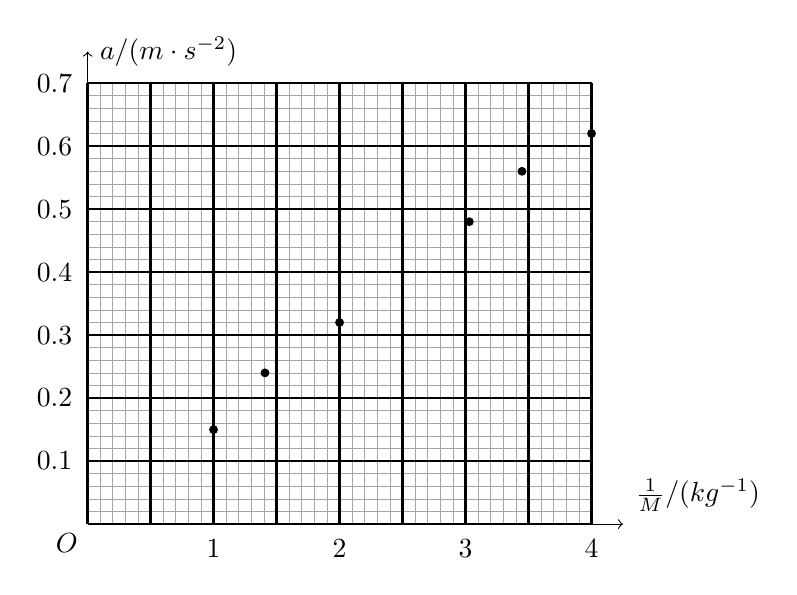
\begin{tikzpicture}[scale=0.8]
	
\draw[gray!70,very thin,step=0.2] (0,0) grid (8,7);
\draw[thick] (0,0) grid (8,7);
\draw [->] (0,0) node [below left]{$ O $}--(8.5,0)  node[above right=1pt] {$ \frac{1}{M}/(kg^{-1}) $} ;
\draw [->] (0,0)--(0,7.5) node[right=1pt] {$ a/(m \cdot s^{-2})  $} ;


\draw (2,0) node[below=2pt] {$ 1 $};
\draw (4,0) node[below=2pt] {$ 2 $};
\draw (6,0) node[below=2pt] {$ 3 $};
\draw (8,0) node[below=2pt] {$ 4 $};


\foreach \x in {1,...,7}
{
	\draw (0,\x) node[left=2pt] {$ 0.\x  $};	
}



\fill (8,6.2) circle [radius=2pt];
\fill (6.8965,5.6) circle [radius=2pt];
\fill (6.06,4.8) circle [radius=2pt];
\fill (4,3.2) circle [radius=2pt];
\fill (2.816,2.4) circle [radius=2pt];
\fill (2,1.5) circle [radius=2pt];

\end{tikzpicture}
\caption{}\label{2020:北京15:2}
\end{figure}




\item 
在探究加速度与力的关系实验之前,需要思考如何测“力”。请在图 \ref{2020:北京15:3} 中画出小车受力的示意图。为了简
化“力”的测量,下列说法正确的是: \underlinegap (选填选项前的字母)
。
\begin{figure}[h!]
\centering
\includesvg[width=0.22\linewidth]{picture/svg/GZ-3-tiyou-0796}
\caption{}\label{2020:北京15:3}
\end{figure}

\fourchoices
{使小车沿倾角合适的斜面运动,小车受力可等效为只受绳的拉力}
{若斜面倾角过大,小车所受合力将小于绳的拉力}
{无论小车运动的加速度多大,砂和桶的重力都等于绳的拉力}
{让小车的运动趋近于匀速运动,砂和桶的重力才近似等于绳的拉力}

\end{enumerate}


\tk{
\begin{enumerate}
%\renewcommand{\labelenumi}{\arabic{enumi}.}
% A(\Alph) a(\alph) I(\Roman) i(\roman) 1(\arabic)
%设定全局标号series=example	%引用全局变量resume=example
%[topsep=-0.3em,parsep=-0.3em,itemsep=-0.3em,partopsep=-0.3em]
%可使用leftmargin调整列表环境左边的空白长度 [leftmargin=0em]
\item
B	
\item 	
如图所示
\begin{center}
%\includesvg[width=0.23\linewidth]{picture/svg/GZ-3-tiyou-0811} 
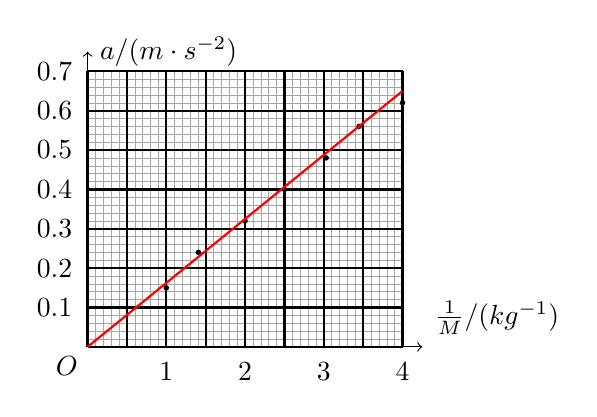
\begin{tikzpicture}[scale=0.5]
	\draw[gray!70,very thin,step=0.2] (0,0) grid (8,7);
	\draw[thick] (0,0) grid (8,7);
	\draw [->] (0,0) node [below left]{$ O $}--(8.5,0)  node[above right=1pt] {$ \frac{1}{M}/(kg^{-1}) $} ;
	\draw [->] (0,0)--(0,7.5) node[right=1pt] {$ a/(m \cdot s^{-2})  $} ;
	
	
	\draw (2,0) node[below=2pt] {$ 1 $};
	\draw (4,0) node[below=2pt] {$ 2 $};
	\draw (6,0) node[below=2pt] {$ 3 $};
	\draw (8,0) node[below=2pt] {$ 4 $};
	
	
	\foreach \x in {1,...,7}
	{
		\draw (0,\x) node[left=2pt] {$ 0.\x  $};	
	}
	
	
	
	\fill (8,6.2) circle [radius=2pt];
	\fill (6.8965,5.6) circle [radius=2pt];
	\fill (6.06,4.8) circle [radius=2pt];
	\fill (4,3.2) circle [radius=2pt];
	\fill (2.816,2.4) circle [radius=2pt];
	\fill (2,1.5) circle [radius=2pt];
	\fill (5,4) circle [radius=2pt];
	\draw[red,thick] (0,0) -- (8,6.5);
\end{tikzpicture}
\end{center}
\item 	
AD
\end{enumerate}
} 


\item 
用图 \ref{2020:北京16:1} 所示的 \subref{2020:北京16:1a} 、 \subref{2020:北京16:1b} 两种方法测量某电源的电动势和内电阻(约为 $ 1 \ \Omega $)
。其中 $ R $ 为电阻箱,电流表的内电阻约
为 $ 0.1 \ \Omega $,电压表的内电阻约为 $ 3 \ k\Omega $。
\begin{figure}[h!]
\centering
\begin{subfigure}{0.4\linewidth}
\centering
\includesvg[width=0.8\linewidth]{picture/svg/GZ-3-tiyou-0797} 
\caption{}\label{2020:北京16:1a}
\end{subfigure}
\hfil
\begin{subfigure}{0.4\linewidth}
\centering
\includesvg[width=0.8\linewidth]{picture/svg/GZ-3-tiyou-0798} 
\caption{}\label{2020:北京16:1b}
\end{subfigure}
\caption{}\label{2020:北京16:1}
\end{figure}

\begin{enumerate}
%\renewcommand{\labelenumi}{\arabic{enumi}.}
% A(\Alph) a(\alph) I(\Roman) i(\roman) 1(\arabic)
%设定全局标号series=example	%引用全局变量resume=example
%[topsep=-0.3em,parsep=-0.3em,itemsep=-0.3em,partopsep=-0.3em]
%可使用leftmargin调整列表环境左边的空白长度 [leftmargin=0em]
\item
利用图 \ref{2020:北京16:1} 中 \subref{2020:北京16:1a} 图实验电路测电源的电动势 $ E $ 和内电阻 $ r $,所测量的实际是图 \ref{2020:北京16:2} 中虚线框所示“等效电源”
的电动势 $ E ^{\prime} $ 和内电阻 $ r ^{\prime} $ 。若电流表内电阻用 $ R_{A} $ 表示,请你用 $ E $、$ r $ 和 $ R_{A} $ 表示出 $ E ^{\prime} $ 、 $ r ^{\prime} $ ,并简要说明理
由。
\begin{figure}[h!]
\centering
\includesvg[width=0.33\linewidth]{picture/svg/GZ-3-tiyou-0799}
\caption{}\label{2020:北京16:2}
\end{figure}



\item 
某同学利用图像分析甲、乙两种方法中由电表内电阻引起的实验误差。在图 \ref{2020:北京16:3} 中,实线是根据实验数据
(图 \subref{2020:北京16:1a} :$ U=IR $,图 \subref{2020:北京16:1b} :$\left.I=\frac{U}{R}\right)$)描点作图得到的 $ U-I $ 图像;虚线是该电源的路端电压 $ U $ 随电流 $ I $ 变化的
$ U-I $ 图像(没有电表内电阻影响的理想情况)。
\begin{figure}[h!]
\centering
\includesvg[width=0.75\linewidth]{picture/svg/GZ-3-tiyou-0800}
%\pfourchoices
%{\includesvg[height=2.2cm]{picture/svg/GZ-3-tiyou-0801}}
%{\includesvg[height=2.2cm]{picture/svg/GZ-3-tiyou-0802}}
%{\includesvg[height=2.2cm]{picture/svg/GZ-3-tiyou-0803}}
%{\includesvg[height=2.2cm]{picture/svg/GZ-3-tiyou-0804}}
\caption{}\label{2020:北京16:3}
\end{figure}




在图 \ref{2020:北京16:3} 中,对应图 \subref{2020:北京16:1a} 电路分析的 $ U-I $ 图像是: \underlinegap ;对应图 \subref{2020:北京16:1b} 电路分析的 $ U-I $ 图像是: \underlinegap 。
\item 
综合上述分析,为了减小由电表内电阻引起的实验误差,本实验应选择图 \ref{2020:北京16:1} 中的 \underlinegap (填“\subref{2020:北京16:1a}”或“\subref{2020:北京16:1b}”)
。

\end{enumerate}


\tk{
\begin{enumerate}
%\renewcommand{\labelenumi}{\arabic{enumi}.}
% A(\Alph) a(\alph) I(\Roman) i(\roman) 1(\arabic)
%设定全局标号series=example	%引用全局变量resume=example
%[topsep=-0.3em,parsep=-0.3em,itemsep=-0.3em,partopsep=-0.3em]
%可使用leftmargin调整列表环境左边的空白长度 [leftmargin=0em]
\item
$E^{\prime}=E $,$ r ^{\prime} =r+R_{\mathrm{A}} $。理由如下:\\
将电源和电流表视为等效电源,电源电动势是电源本身具有的属性,电流表不具有产生电动
势的本领,所以等效电源的电动势仍然为
$E^{\prime}=E $,
而电流表的内阻和电动势的内阻作为等效电源的内阻,即$ r ^{\prime} =r+R_{\mathrm{A}} $。
\item 
C \quad A
\item 
\subref{2020:北京16:1b}
\end{enumerate}
} 


\gaokaojs

\item
无人机在距离水平地面高度 $ h $ 处,以速度 $ v_{0} $ 水平匀速飞行并释放一包裹,不计空气阻力,重力加速度为 $ g $。
\begin{enumerate}
%\renewcommand{\labelenumi}{\arabic{enumi}.}
% A(\Alph) a(\alph) I(\Roman) i(\roman) 1(\arabic)
%设定全局标号series=example	%引用全局变量resume=example
%[topsep=-0.3em,parsep=-0.3em,itemsep=-0.3em,partopsep=-0.3em]
%可使用leftmargin调整列表环境左边的空白长度 [leftmargin=0em]
\item
求包裹释放点到落地点的水平距离 $ x $;
\item 
求包裹落地时的速度大小 $ v $;
\item 
以释放点为坐标原点,初速度方向为 $ x $ 轴方向,竖直向下为 $ y $ 轴方向,建立平面直角坐标系,写出该包
裹运动的轨迹方程。
\end{enumerate}




\banswer{
\begin{enumerate}
%\renewcommand{\labelenumi}{\arabic{enumi}.}
% A(\Alph) a(\alph) I(\Roman) i(\roman) 1(\arabic)
%设定全局标号series=example	%引用全局变量resume=example
%[topsep=-0.3em,parsep=-0.3em,itemsep=-0.3em,partopsep=-0.3em]
%可使用leftmargin调整列表环境左边的空白长度 [leftmargin=0em]
\item
$x=v_{0} \sqrt{\frac{2 h}{g}}$
\item 
$v=\sqrt{v_{0}^{2}+2 g h}$
\item 
$y=\frac{g}{2 v_{0}^{2}} x^{2}$
\end{enumerate}
}


\vfill

\item
如图 \subref{2020:北京18:a} 所示, $ N =200 $ 匝的线圈(图中只画了 $ 2 $ 匝),电阻 $ r=2 \ \Omega $ ,其两端与一个 $ R = 48 \ \Omega $ 的电阻相连,线
圈内有指向纸内方向的磁场。线圈中的磁通量按图 \subref{2020:北京18:b} 所示规律变化。
\begin{enumerate}
%\renewcommand{\labelenumi}{\arabic{enumi}.}
% A(\Alph) a(\alph) I(\Roman) i(\roman) 1(\arabic)
%设定全局标号series=example	%引用全局变量resume=example
%[topsep=-0.3em,parsep=-0.3em,itemsep=-0.3em,partopsep=-0.3em]
%可使用leftmargin调整列表环境左边的空白长度 [leftmargin=0em]
\item
判断通过电阻 $ R $ 的电流方向;
\item 
求线圈产生的感应电动势 $ E $;
\item 
求电阻 $ R $ 两端的电压 $ U $。
\end{enumerate}
\begin{figure}[h!]
\flushright
\begin{subfigure}{0.3\linewidth}
\centering
\includesvg[width=0.87\linewidth]{picture/svg/GZ-3-tiyou-0805} 
\caption{}\label{2020:北京18:a}
\end{subfigure}
\begin{subfigure}{0.3\linewidth}
\centering
\includesvg[width=0.87\linewidth]{picture/svg/GZ-3-tiyou-0806} 
\caption{}\label{2020:北京18:b}
\end{subfigure}
\end{figure}


\banswer{
\begin{enumerate}
%\renewcommand{\labelenumi}{\arabic{enumi}.}
% A(\Alph) a(\alph) I(\Roman) i(\roman) 1(\arabic)
%设定全局标号series=example	%引用全局变量resume=example
%[topsep=-0.3em,parsep=-0.3em,itemsep=-0.3em,partopsep=-0.3em]
%可使用leftmargin调整列表环境左边的空白长度 [leftmargin=0em]
\item
$a \rightarrow b$
\item 
$ E=10 \ V $
\item 
$ U=9.6 \ V $
\end{enumerate}
}




\newpage
\item 
如图 \subref{2020:北京19:a} 所示,真空中有一长直细金属导线 $ MN $,与导线同轴放置一半径为 $ R $ 的金属圆柱面。假设导线沿径向均
匀射出速率相同的电子,已知电子质量为 $ m $,电荷量为 $ e $。不考虑出射电子间的相互作用。
\begin{enumerate}
%\renewcommand{\labelenumi}{\arabic{enumi}.}
% A(\Alph) a(\alph) I(\Roman) i(\roman) 1(\arabic)
%设定全局标号series=example	%引用全局变量resume=example
%[topsep=-0.3em,parsep=-0.3em,itemsep=-0.3em,partopsep=-0.3em]
%可使用leftmargin调整列表环境左边的空白长度 [leftmargin=0em]
\item
可以用以下两种实验方案测量出射电子的初速度:
\begin{enumerate}
	%\renewcommand{\labelenumi}{\arabic{enumi}.}
	% A(\Alph) a(\alph) I(\Roman) i(\roman) 1(\arabic)
	%设定全局标号series=example	%引用全局变量resume=example
	%[topsep=-0.3em,parsep=-0.3em,itemsep=-0.3em,partopsep=-0.3em]
	%可使用leftmargin调整列表环境左边的空白长度 [leftmargin=0em]
	\item
在柱面和导线之间,只加恒定电压;

\item 
在柱面内,只加与 $ MN $ 平行的匀强磁场。
\end{enumerate}


当电压为 $ U_{0} $ 或磁感应强度为 $ B_{0} $ 时,刚好没有电子到达柱面。分别计算出射电子的初速度 $ v_{0} $。

\item 
撤去柱面,沿柱面原位置放置一个弧长为 $ a $、长度为 $ b $ 的金属片,如图 \subref{2020:北京19:b} 所示。在该金属片上检测到出
射电子形成的电流为 $ I $ ,电子流对该金属片的压强为 $ p $。求单位长度导线单位时间内出射电子的总动能。

\end{enumerate}
\begin{figure}[h!]
\flushright
\begin{subfigure}{0.3\linewidth}
\centering
\includesvg[width=0.5\linewidth]{picture/svg/GZ-3-tiyou-0807} 
\caption{}\label{2020:北京19:a}
\end{subfigure}
\begin{subfigure}{0.3\linewidth}
\centering
\includesvg[width=0.5\linewidth]{picture/svg/GZ-3-tiyou-0808} 
\caption{}\label{2020:北京19:b}
\end{subfigure}
\end{figure}


\banswer{
\begin{enumerate}
%\renewcommand{\labelenumi}{\arabic{enumi}.}
% A(\Alph) a(\alph) I(\Roman) i(\roman) 1(\arabic)
%设定全局标号series=example	%引用全局变量resume=example
%[topsep=-0.3em,parsep=-0.3em,itemsep=-0.3em,partopsep=-0.3em]
%可使用leftmargin调整列表环境左边的空白长度 [leftmargin=0em]
\item
\begin{enumerate}
	%\renewcommand{\labelenumi}{\arabic{enumi}.}
	% A(\Alph) a(\alph) I(\Roman) i(\roman) 1(\arabic)
	%设定全局标号series=example	%引用全局变量resume=example
	%[topsep=-0.3em,parsep=-0.3em,itemsep=-0.3em,partopsep=-0.3em]
	%可使用leftmargin调整列表环境左边的空白长度 [leftmargin=0em]
	\item
当电压为$ U_{0} $时$v_{0}=\sqrt{\frac{2 e U_{0}}{m}}$
\item 
磁感应强度为$ B_{0} $时$v_{0}=\frac{B_{0} q R}{2 m}$(粒子的运动轨迹在水平面内)
\end{enumerate}
\item 
$\frac{e \pi ab   p^{2} R}{m I}$
\end{enumerate}
}



\newpage
\item 
某试验列车按照设定的直线运动模式,利用计算机控制制动装置,实现安全准确地进站停车。制动装置包括电
气制动和机械制动两部分。图 \subref{2020:北京20:a} 所示为该列车在进站停车过程中设定的加速度大小 $ a $车 随速度 $ v $ 的变化曲线。
\begin{enumerate}
%\renewcommand{\labelenumi}{\arabic{enumi}.}
% A(\Alph) a(\alph) I(\Roman) i(\roman) 1(\arabic)
%设定全局标号series=example	%引用全局变量resume=example
%[topsep=-0.3em,parsep=-0.3em,itemsep=-0.3em,partopsep=-0.3em]
%可使用leftmargin调整列表环境左边的空白长度 [leftmargin=0em]
\item
求列车速度从 $ 20 \ m/s $ 降至 $ 3 \ m/s $ 经过的时间 $ t $ 及行进的距离 $ x $。
\item 
有关列车电气制动,可以借助图 \subref{2020:北京20:b} 模型来理解。图中水平平行金属导轨处于竖直方向的匀强磁场中,回
路中的电阻阻值为 $ R $,不计金属棒 $ MN $ 及导轨的电阻。 $ MN $ 沿导轨向右运动的过程,对应列车的电气制
动过程,可假设 $ MN $ 棒运动的速度与列车的速度、棒的加速度与列车电气制动产生的加速度成正比。列
车开始制动时,其速度和电气制动产生的加速度大小对应图 $ 1 $ 中的 $ P $ 点。论证电气制动产生的加速度大
小随列车速度变化的关系,并在图 \subref{2020:北京20:a}中画出图线。

\item 
制动过程中,除机械制动和电气制动外,列车还会受到随车速减小而减小的空气阻力。分析说明列车从$ 100 \ m/s $ 减到 $ 3 \ m/s $ 的过程中,在哪个速度附近所需机械制动最强?


\end{enumerate}
\begin{figure}[h!]
\flushright 
\begin{subfigure}{0.45\linewidth}
\centering
\includesvg[width=0.97\linewidth]{picture/svg/GZ-3-tiyou-0809}
\caption{}\label{2020:北京20:a}
\end{subfigure}
\begin{subfigure}{0.4\linewidth}
\centering
\includesvg[width=0.95\linewidth]{picture/svg/GZ-3-tiyou-0810} 
\caption{}\label{2020:北京20:b}
\end{subfigure}
\end{figure}

\banswer{
\begin{enumerate}
%\renewcommand{\labelenumi}{\arabic{enumi}.}
% A(\Alph) a(\alph) I(\Roman) i(\roman) 1(\arabic)
%设定全局标号series=example	%引用全局变量resume=example
%[topsep=-0.3em,parsep=-0.3em,itemsep=-0.3em,partopsep=-0.3em]
%可使用leftmargin调整列表环境左边的空白长度 [leftmargin=0em]
\item
$t=\frac{170}{7} = \approx 24.3 \ s $\\
$ x = \frac{1955}{7} = \approx 279.3 \ m$
\item 
列车电气制动产生的加速度与列车的速度成正比,为过$ P $ 点的
正比例函数,论证过程略。画出的图线如下图所示:
\begin{center}
 \includesvg[width=0.93\linewidth]{picture/svg/GZ-3-tiyou-0813} 
\end{center}
\item 
由于空气阻力造成的加速度和电气制动造成的加速度之和依然与速度成正比关系,易知在$ 3 \ m/s $附近所需的机械制动最强。
\end{enumerate}
}



\end{enumerate}

